\documentclass[12pt]{ruthesis}
\usepackage{amsmath}
\usepackage{amssymb}
\usepackage{latexsym}
\usepackage{graphics}
\usepackage{epsfig,epsf,rotating}
\usepackage{subfigure}
%\usepackage{pictex}
\usepackage{epsf}
%\usepackage{cite}
\usepackage{theorem}
\newtheorem{proposition}{Proposition}

\theoremheaderfont{\itshape} {\theoremstyle{break}
\newtheorem{Fact}{Fact}[chapter]} \theoremstyle{break}
\newtheorem{Lem}{Lemma}[chapter] \theoremstyle{break}
\newtheorem{Thm}{Theorem}[chapter] {\theoremstyle{plain}
  \theorembodyfont{\rmfamily}  \newtheorem{Prf}{Proof}[chapter]}
{\theoremstyle{plain}
  \theorembodyfont{\rmfamily}  \newtheorem{Def}{Definition}[chapter]}

\title{Search for Stop Quark via All-Hadronic Decay Channels}
\ctitle{Search for Stop Quark via All-Hadronic Decay Channels}
\author{Matthew Cavenaugh Kilpatrick}
\department{Physics and Astronomy}
\school{Rice University}
\degree{Doctor of Philosophy}

\committee {
        Karl Ecklund, Chair \\
        Associate Professor of Physics and Astronomy \and
        Paul Padley \\
        Professor of Physics and Astronomy \and
        David Scott\\
        Noah Harding Professor
}

\address{Houston, Texas}
\donemonth{April} \doneyear{2019} \makeindex
\begin{document}

  \begin{frontmatter}
   \pagenumbering{roman}
   %\makecover
   \maketitle
   \thispagestyle{empty}
\begin{abstract}
A search for the top squark from direct production via the all-hadronic decay channel is performed on 136.7 $\text{fb}^{-1}$ at a center-of-mass energy of 13 TeV from Run 2 of the LHC. Events are categorized into exclusive regions designed to optimize the different search topologies of the analysis. The analysis concentrates on identifying heavy objects such as top quarks and W boson, from their decays using a custom tagger for resolved tops and multivariate methods for others. A low $\Delta m$ spectra is enhanced using the soft $b$ quark jet transverse momentum which is typical of signal in a boosted regime with initial-state radiation. We then provide exclusion limits for each signal in the simplified models with multiple decay products.
\end{abstract}



   %\include{ack}
   \tableofcontents
   \listoffigures
   \listoftables
%   \include{ded}
  \end{frontmatter}
\pagenumbering{arabic}

\linespacing{1.7}

\chapter{Introduction}
\label{ch:Intro}

The Standard Model (SM) is a robust framework that allows for accurate predictions of processes involving the interactions of elementary particles. It has been developed over the course of many decades, which involved many additions such as three generations of quarks and leptons and the combination of Electromagnetism and the Weak force into a single theory. Unfortunately, we have evidence that is not explained by the SM and has eluded physicists for many years. We intend to do a search for a potential particle beyond the current SM.

\section{Motivation}
\label{sec:Motivation}

Through various methods of experiment, we have seen that the current knowledge of elementary particles in the SM do not explain all of the known matter in the universe. Due to galactic velocity rotational curves we can deduce that the mass of galaxies must be much more than the visible matter that can be measured. This "dark matter" must act quite weakly with the three forces of the SM, but can still be quite important for gravitational effects. There are many theories beyond the SM that can explain these effects, but we will concentrate on Supersymmetry (SUSY) because of the potential for a dark matter candidate, a solution to the Hierarchy problem, and a potential Grand Unified Theory (GUT).

SUSY allows for every fermion to have a bosonic partner, and vice-versa, which has all of the same quantum numbers except for a difference of $\frac{1}{2}$-integer spin. We know that since it has not yet been found that the theory must be a broken symmetry, such that the masses of the SUSY partners must have a higher mass than the SM particle. One of the main aspects of SUSY, is the conservation of $R$-parity, which implies the existence of a Lightest Supersymmetric Particle (LSP). This LSP could be a potential dark matter candidate since it is stable and weakly interacting. 

The Hierarchy problem is due to the loop interactions of massive quarks with the Higgs boson. This coupling causes a quadratic divergence of the Higgs mass, $m_H$, and can only be renormalized by fine tuning the coupling parameters. A potential solution is the coupling of an additional bosonic particle to the quarks. This additional coupling allows for a cancellation of quadratic divergence into a logarithmic divergence, which is then renormalizable by the normal methods. This can renormalize the mass of the Higgs boson to the known value of $m_H=125.18$ \GeV{} that was discovered in 2012. Finally, SUSY also allows for a mechanism for a potential GUT. The additional superpartners allow for the three forces of the SM to converge at a large energy scale of the order $10^{16}$ GeV. We now need to develop a search strategy to try and detect these potential SUSY particles.

\section{Search}
\label{sec:search}

There are many possible searches for SUSY particles. In the Minimal Supersymmetric Standard Model (MSSM), it can be determined that the lightest squark that can be produced at the Large Hadron Collider (LHC) is the stop, \st{}, which will then decay into SM particles and the LSP.  We are developing an all-hadronic search to find the \st{} which will be as inclusive as possible, so we will include all possible decay modes to get additional limits or possible detection. 

Due to the all hadronic aspect of the decay, the main backgrounds are caused by, a lost lepton due to a lepton passing the kinematic cuts of the detector, \Znunu{} background where the missing energy is caused by the neutrinos escaping the detector, Quantum Chromodynamics (QCD) background which can be caused by the mis-measurement of jets in the event, and a rare background caused by many different types of processes which are estimated by a three lepton method of identification. We have developed 183 search regions to look for the top squark, \st{}. This is then used to get a statistical estimation of the limits on the cross-section for each of the processes that we are interested in searching. In the following chapters, we will: look into the derivation of the SM and motivations for SUSY; provide a description of the Compact Muon Solenoid (CMS) detector and the various subdetectors; next the description of the object selection and search strategy for the analysis; the methods of each individual background are described; and the description and analysis of the results and limits. 



\appendix

%\chapter{Tau Multivariate Analysis}\label{sec:TauMVA}

The identification of taus that decay hadronically has been under extensive study to distinguish whether the custom tau multivariate analysis (tauMVA), the isolated track (isotrack) method, or the MVA from that is provided by the tau POG (tauPOG). The custom tauMVA was trained on PF charged hadron candidates with $\pt>10~\GeV$ and $|\eta|<2.4$ along with an additional PF photon candidate, if any, with highest $\pt>0.5!\GeV$ and within a cone of $\Delta R\leq0.2$ of the charged hadron candidate. The tau candidate is also required to have a transverse mass $m_T(\tau_h,\met)<100~\GeV$, where $m_T(\tau_h,\met)$ is defined as follows,
\begin{equation}\label{tauMT}
m_T(\tau_h,\met)=\sqrt{2\cdot\pt(\tau_h+\text{nearest}\gamma)\cdot\met\cdot(1-\cos\Delta\phi)}.
\end{equation}

The addition of photons in the final definition is due to the possibility of taus decaying to neutral pions. This improves the resolution for the hadronic tau candidate. The inputs for the MVA are as follows:
\begin{itemize}
	\item The \pt and $|\eta|$ of the $\tau$ candidate.
	\item The sum \pt of charged particles associated to the primary vertex within $\Delta R$ cones of sizes 0.1, 0.2, 0.3, and 0.4 around the $\tau$ candidate.
	\item The summed \pt of all particles within $\Delta R$ cones of sizes 0.1, 0.2, 0.3, and 0.4 around the candidate, now including the neutral contribution from pileup particles, which is reduced by applying the $\Delta \beta$ correction to the neutral component of the isolation quantity. 
	\item The distance in $\Delta R$ to the nearest charged PF candidate with $\pt>1~\GeV$.
	\item The distance in $\Delta R$ to the axis of the jet containing the $\tau$ candidate, and the b-tagging discriminant (DeepCSV) value for the jet, provided that the jet has $\pt>30~\GeV$ and $|\eta|<2.4$.
\end{itemize}

\begin{figure}
 	\centering
	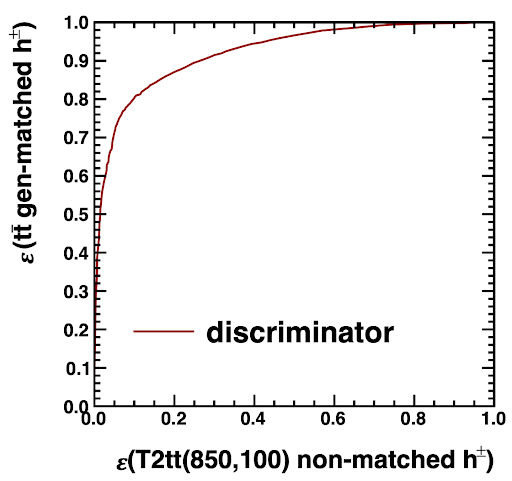
\includegraphics[width=0.60\textwidth]{tauMVA_ROCCurve.png}
 	\caption[Tau MVA ROC Curve]{A Reciever operator characteristic curve for the tauMVA discriminator.}
 	\label{tauMVAROCCurve} 
\end{figure}

\begin{figure}[!htb]
	\begin{center}
		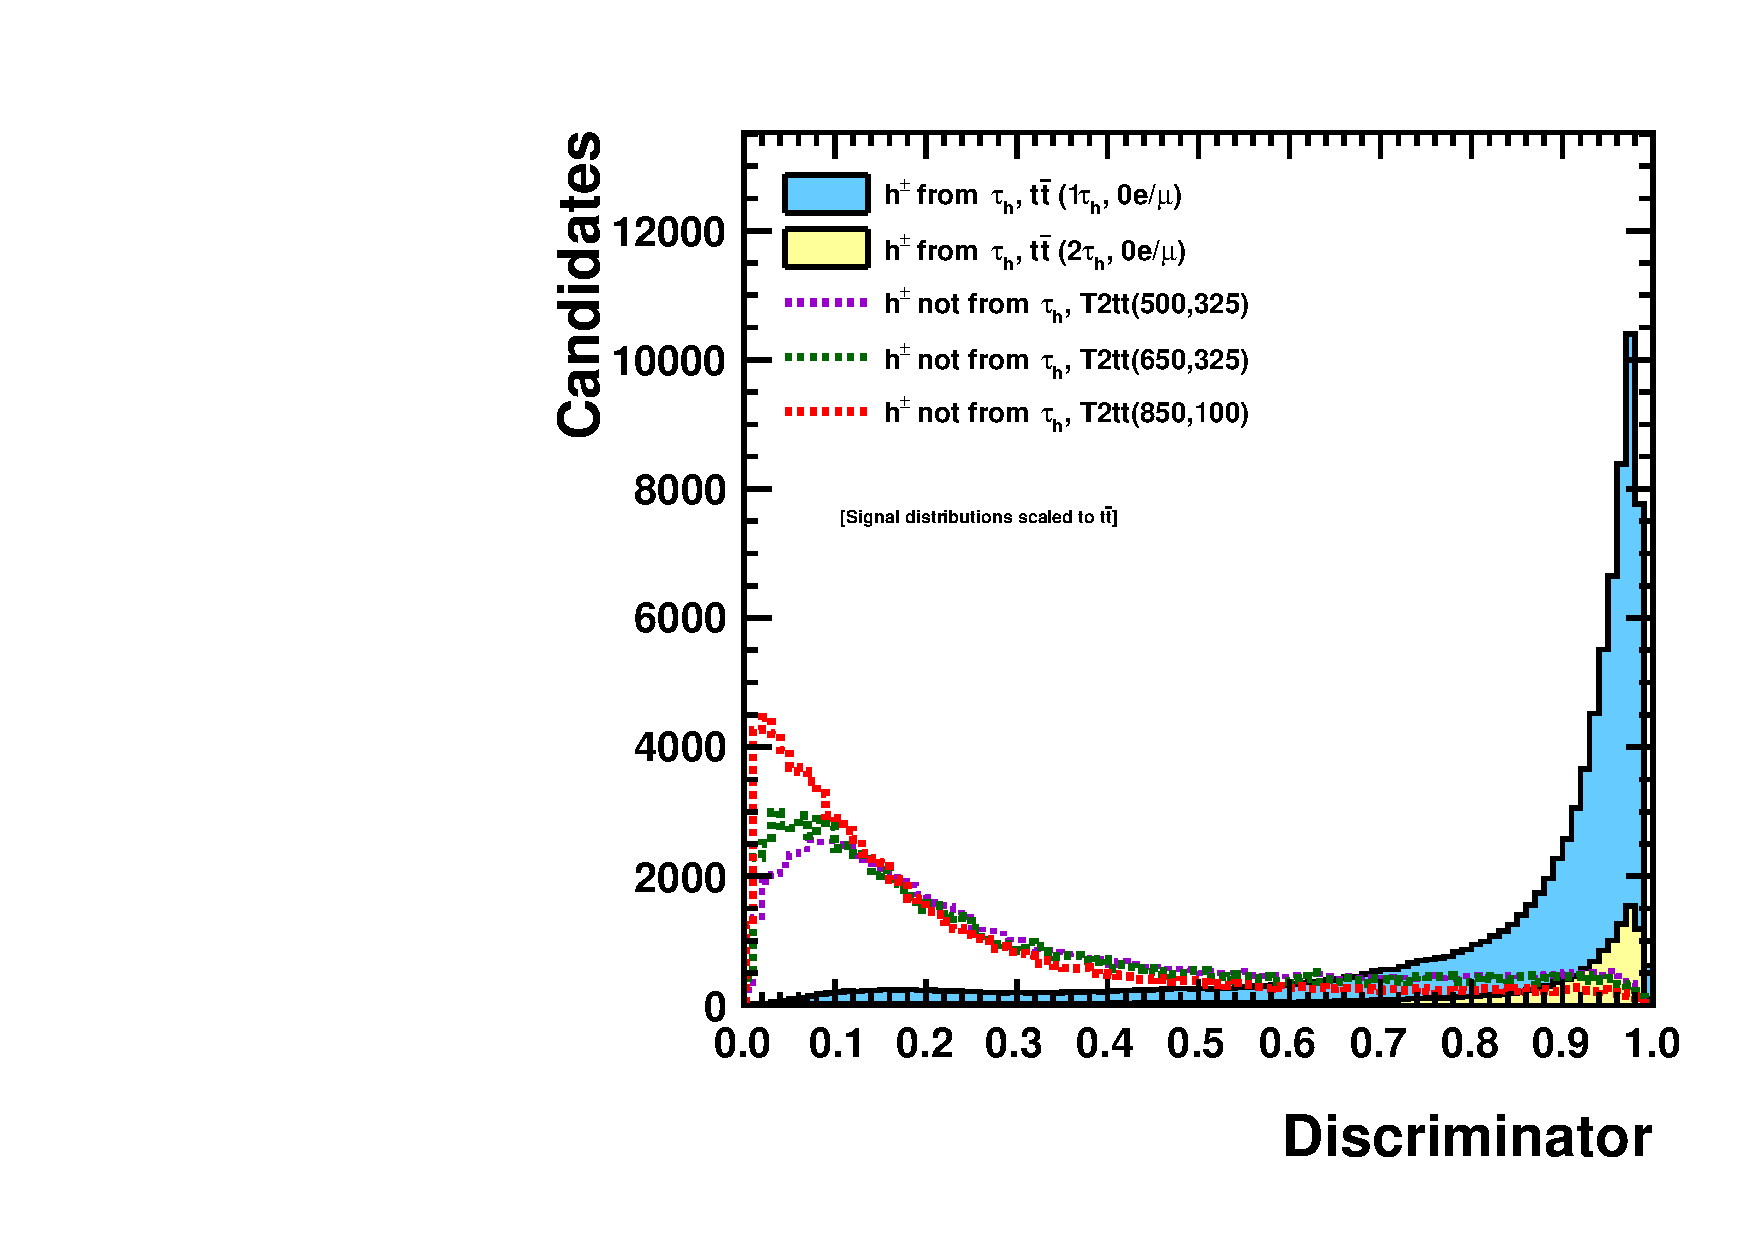
\includegraphics[width=0.5\textwidth]{mva_eta03_sigscalesumbkg_thesis.pdf}
		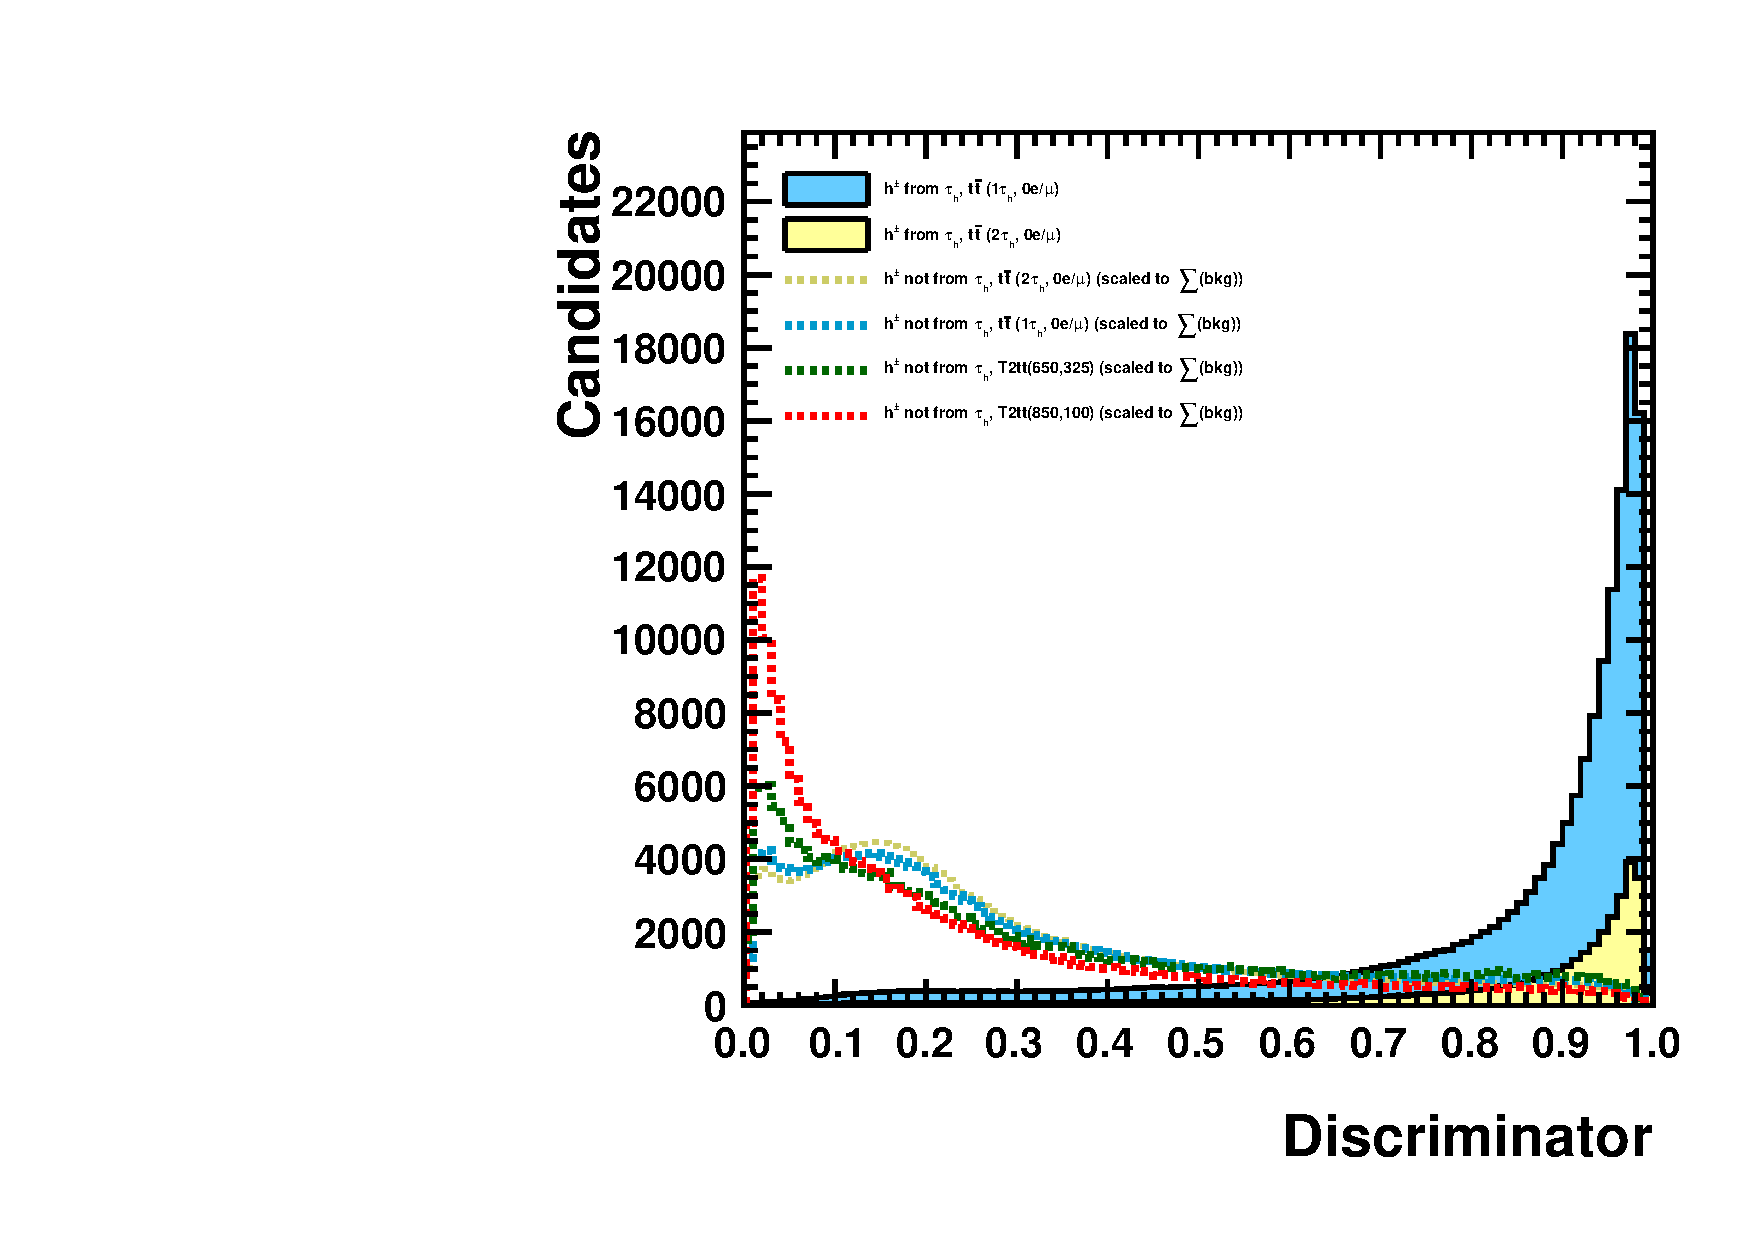
\includegraphics[width=0.5\textwidth]{mva_fakett_eta03_allpu_sigscalesumbkg_thesis.pdf} \\
	\end{center}
	\caption[Tau MVA Discriminator]{Tau MVA discriminator for different types of samples.
	}
	\label{fig:tau-discriminator}
\end{figure}

% matches pred table
% copy and paste the output from the end of LLBPred() (it calls printMoriond17Table) between the below labels "start insert" and "stop insert".
\begin{table}[!h]
\begin{center}
\resizebox*{\textwidth}{!}{
\begin{tabular}{|c||c||c|c|c||c|c|c|}
\hline
& & \multicolumn{3}{c||}{\ttbar{} 1-lepton} & \multicolumn{3}{c||}{\ttbar{} Di-lepton}\\
\hline
\hline
Type & Discriminator Cut & Efficiency & Fake Rate & Efficiency/Fake & Efficiency & Fake Rate & Efficiency/Fake \\
\hline
IsoTrack  & - & 27.9 \% & 6.1 \% & 4.541 & 24.8 \% & 6.1 \% & 4.084 \\
TauMVA & 0.68  & 34.9 \% & 6.9 \% & 5.046 & 24.7 \% & 5.3 \% & 4.689 \\
TauMVA & 0.70  & 34.6 \% & 6.5 \% & 5.355 & 24.4 \% & 4.9 \% & 4.997 \\
TauMVA & 0.71  & 34.4 \% & 6.2 \% & 5.525 & 24.2 \% & 4.7 \% & 5.170 \\
TauMVA & 0.73  & 33.9 \% & 5.7 \% & 5.914 & 23.8 \% & 4.3 \% & 5.540 \\
TauMVA & 0.74  & 33.6 \% & 5.5 \% & 6.119 & 23.6 \% & 4.1 \% & 5.712 \\
TauMVA & 0.75  & 33.4 \% & 5.2 \% & 6.356 & 23.4 \% & 3.9 \% & 5.961 \\
\hline 
\end{tabular}
}
\caption[TauMVA Background Optimization]{\label{tab:tau-mva-bkg}Comparing the efficiencies and Fake Rates of many difference discriminator cuts for the TauMVA and IsoTrack methods with SM simulation.}
\end{center}
\end{table}

\begin{table}[!h]
\begin{center}
\resizebox*{\textwidth}{!}{
\begin{tabular}{|c||c||c|c|c||c|c|c|}
\hline
& & \multicolumn{3}{c||}{T1tttt(2000,100)} & \multicolumn{3}{c||}{T2tt(850,100)}\\
\hline
\hline
Type & Discriminator Cut & Efficiency & Fake Rate & Efficiency/Fake & Efficiency & Fake Rate & Efficiency/Fake \\
\hline
IsoTrack  & - & 7.4 \% & 2.9 \% & 2.503 & 5.5 \% & 2.0 \% & 2.704 \\
TauMVA & 0.68  & 5.7 \% & 8.1 \% & 0.696 & 4.8 \% & 4.7 \% & 1.017 \\
TauMVA & 0.70  & 5.5 \% & 7.5 \% & 0.735 & 4.7 \% & 4.4 \% & 1.075 \\
TauMVA & 0.71  & 5.5 \% & 7.2 \% & 0.760 & 4.7 \% & 4.2 \% & 1.102 \\
TauMVA & 0.73  & 5.4 \% & 6.6 \% & 0.806 & 4.6 \% & 3.9 \% & 1.175 \\
TauMVA & 0.74  & 5.3 \% & 6.3 \% & 0.832 & 4.5 \% & 3.7 \% & 1.214 \\
TauMVA & 0.75  & 5.2 \% & 6.0 \% & 0.869 & 4.5 \% & 3.5 \% & 1.262 \\
\hline 
\end{tabular}
}
\caption[TauMVA Signal Optimization]{\label{tab:tau-mva-sig}Comparing the efficiencies and Fake Rates of many difference discriminator cuts for the TauMVA and IsoTrack methods with two SUSY simulations.}
\end{center}
\end{table}

\begin{table}[!h]
\begin{center}
\resizebox*{\textwidth}{!}{
\begin{tabular}{|c||c|c||c|c||c|c|}
\hline
& \multicolumn{2}{c||}{\ttbar{} 1-lepton} & \multicolumn{2}{c||}{T1tttt(2000,100)} & \multicolumn{2}{c|}{T2tt(850,100)} \\
\hline
\hline
Methods & Veto Percentage & Veto Efficiency & Veto Percentage & Veto Efficiency & Veto Percentage & Veto Efficiency \\
\hline
TauMVA         & 32.2\% & 57.7\% & 12.9 \% & 10.7 \% & 6.5\% & 10.9 \%  \\
IsoTrack        & 21.3 \% & 37.9 \% & 4.4 \% & 2.5 \% & 2.6 \% & 6.6 \%  \\
TauPOG         & 171 \% & 29.7 \% & 7.0 \% & 3.2 \%	& 5.2 \% & 2.5 \% \\
IsoTrack + TauPOG & 29.0 \% & 49.1 \% & 10.4 \% & 5.6 \% & 7.2 \% & 22.6 \% \\
\hline 

\end{tabular}
}
\caption[Tau Identification Comparisons]{\label{tab:tau-comparisons}Comparing the veto percentage and efficiency for the TauMVA, IsoTrack, TauPOG, and the IsoTrack + TauPOG methods with SM and SUSY simulations.}
\end{center}
\end{table}


Now that we have the definition for the TauMVA and have trained it on our samples to identify hadronically decaying taus. We want to compare the veto efficiencies and fake rates of the each method: TauMVA, IsoTrack, TauPOG, or a combination of IsoTrack and TauPOG. In Table \ref{tab:tau-comparisons}
%\appendix
%\addcontentsline{toc} {chapter}{\numberline {}Appendix A}
%\chapter{Tau Multivariate Analysis}\label{sec:TauMVA}

The identification of taus that decay hadronically has been under extensive study to distinguish whether the custom tau multivariate analysis (tauMVA), the isolated track (isotrack) method, or the MVA from that is provided by the tau POG (tauPOG). The custom tauMVA was trained on PF charged hadron candidates with $\pt>10~\GeV$ and $|\eta|<2.4$ along with an additional PF photon candidate, if any, with highest $\pt>0.5!\GeV$ and within a cone of $\Delta R\leq0.2$ of the charged hadron candidate. The tau candidate is also required to have a transverse mass $m_T(\tau_h,\met)<100~\GeV$, where $m_T(\tau_h,\met)$ is defined as follows,
\begin{equation}\label{tauMT}
m_T(\tau_h,\met)=\sqrt{2\cdot\pt(\tau_h+\text{nearest}\gamma)\cdot\met\cdot(1-\cos\Delta\phi)}.
\end{equation}

The addition of photons in the final definition is due to the possibility of taus decaying to neutral pions. This improves the resolution for the hadronic tau candidate. The inputs for the MVA are as follows:
\begin{itemize}
	\item The \pt and $|\eta|$ of the $\tau$ candidate.
	\item The sum \pt of charged particles associated to the primary vertex within $\Delta R$ cones of sizes 0.1, 0.2, 0.3, and 0.4 around the $\tau$ candidate.
	\item The summed \pt of all particles within $\Delta R$ cones of sizes 0.1, 0.2, 0.3, and 0.4 around the candidate, now including the neutral contribution from pileup particles, which is reduced by applying the $\Delta \beta$ correction to the neutral component of the isolation quantity. 
	\item The distance in $\Delta R$ to the nearest charged PF candidate with $\pt>1~\GeV$.
	\item The distance in $\Delta R$ to the axis of the jet containing the $\tau$ candidate, and the b-tagging discriminant (DeepCSV) value for the jet, provided that the jet has $\pt>30~\GeV$ and $|\eta|<2.4$.
\end{itemize}

\begin{figure}
 	\centering
	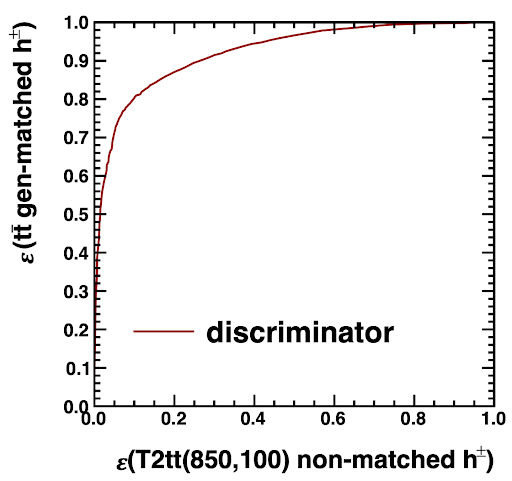
\includegraphics[width=0.60\textwidth]{tauMVA_ROCCurve.png}
 	\caption[Tau MVA ROC Curve]{A Reciever operator characteristic curve for the tauMVA discriminator.}
 	\label{tauMVAROCCurve} 
\end{figure}

\begin{figure}[!htb]
	\begin{center}
		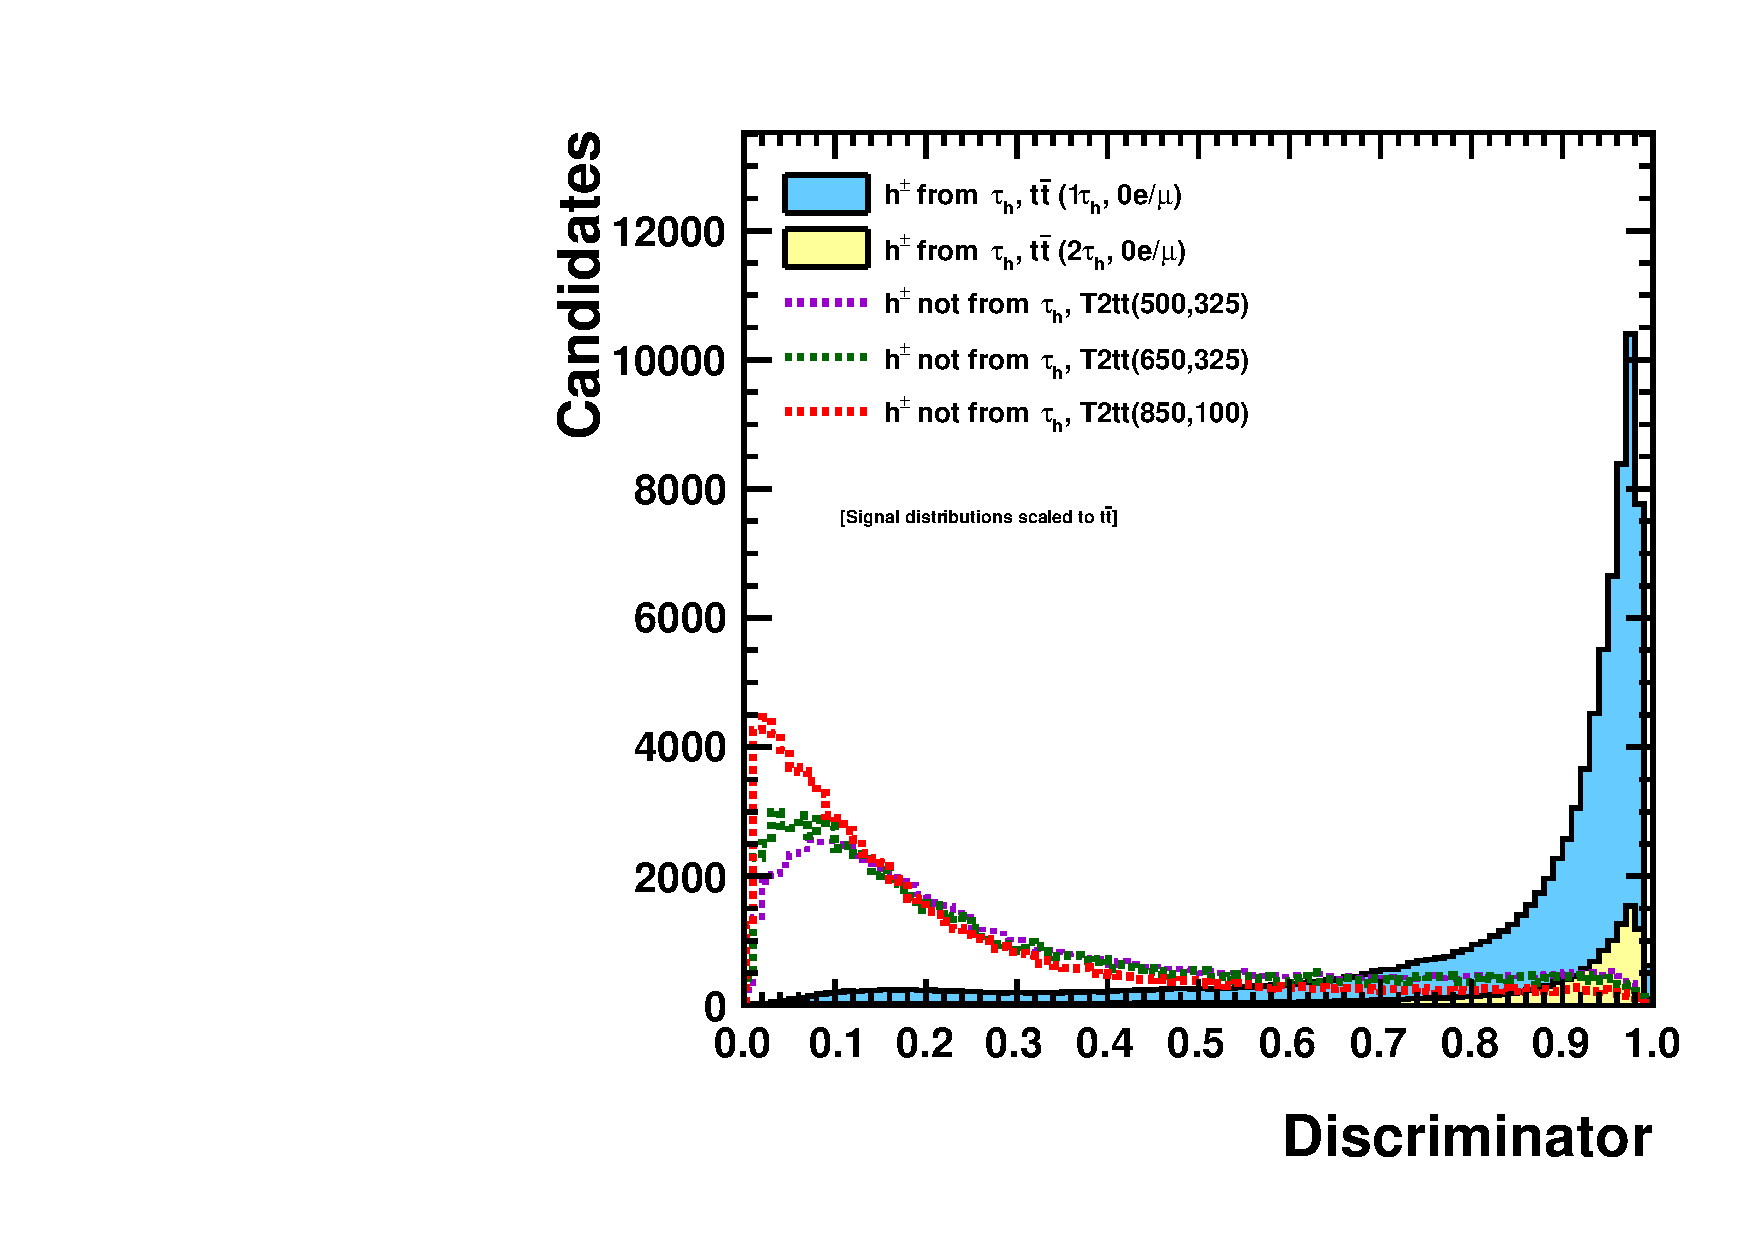
\includegraphics[width=0.5\textwidth]{mva_eta03_sigscalesumbkg_thesis.pdf}
		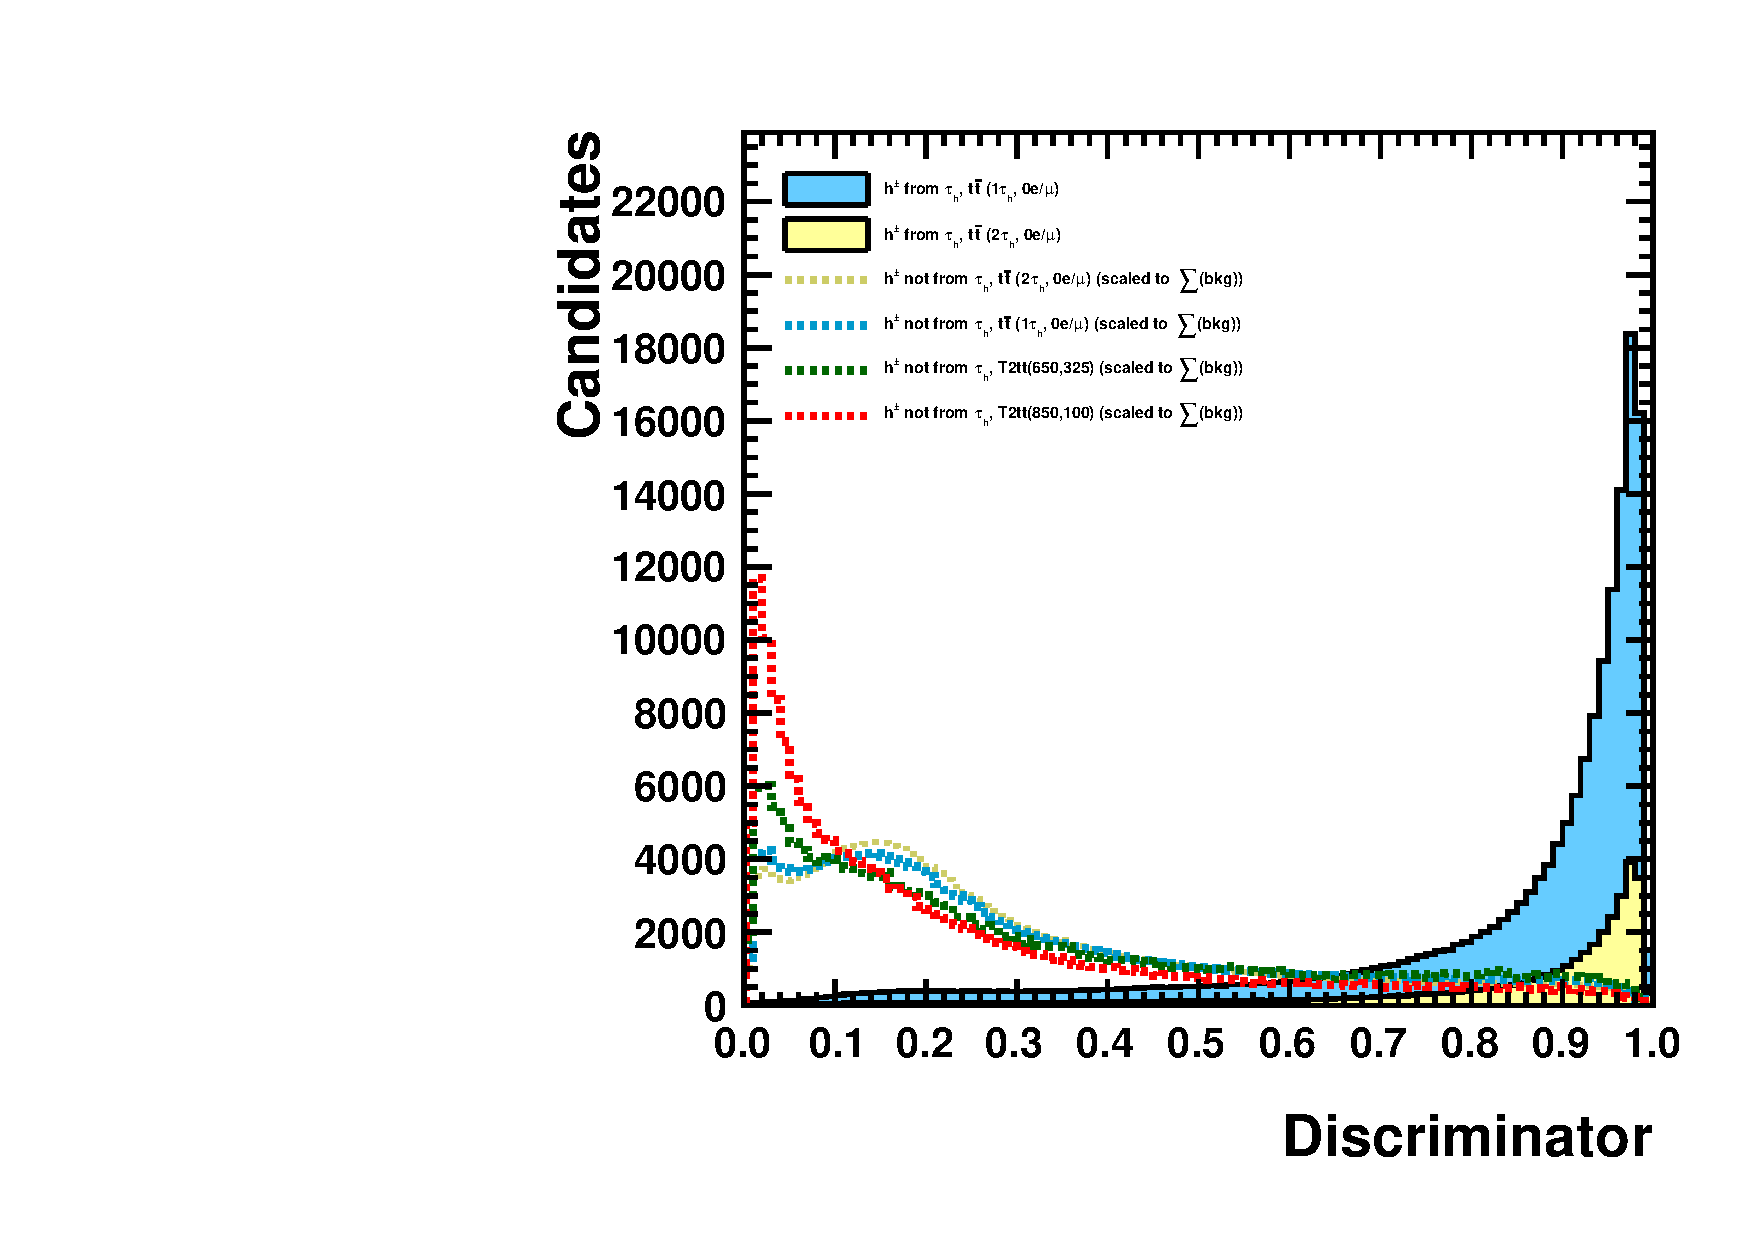
\includegraphics[width=0.5\textwidth]{mva_fakett_eta03_allpu_sigscalesumbkg_thesis.pdf} \\
	\end{center}
	\caption[Tau MVA Discriminator]{Tau MVA discriminator for different types of samples.
	}
	\label{fig:tau-discriminator}
\end{figure}

% matches pred table
% copy and paste the output from the end of LLBPred() (it calls printMoriond17Table) between the below labels "start insert" and "stop insert".
\begin{table}[!h]
\begin{center}
\resizebox*{\textwidth}{!}{
\begin{tabular}{|c||c||c|c|c||c|c|c|}
\hline
& & \multicolumn{3}{c||}{\ttbar{} 1-lepton} & \multicolumn{3}{c||}{\ttbar{} Di-lepton}\\
\hline
\hline
Type & Discriminator Cut & Efficiency & Fake Rate & Efficiency/Fake & Efficiency & Fake Rate & Efficiency/Fake \\
\hline
IsoTrack  & - & 27.9 \% & 6.1 \% & 4.541 & 24.8 \% & 6.1 \% & 4.084 \\
TauMVA & 0.68  & 34.9 \% & 6.9 \% & 5.046 & 24.7 \% & 5.3 \% & 4.689 \\
TauMVA & 0.70  & 34.6 \% & 6.5 \% & 5.355 & 24.4 \% & 4.9 \% & 4.997 \\
TauMVA & 0.71  & 34.4 \% & 6.2 \% & 5.525 & 24.2 \% & 4.7 \% & 5.170 \\
TauMVA & 0.73  & 33.9 \% & 5.7 \% & 5.914 & 23.8 \% & 4.3 \% & 5.540 \\
TauMVA & 0.74  & 33.6 \% & 5.5 \% & 6.119 & 23.6 \% & 4.1 \% & 5.712 \\
TauMVA & 0.75  & 33.4 \% & 5.2 \% & 6.356 & 23.4 \% & 3.9 \% & 5.961 \\
\hline 
\end{tabular}
}
\caption[TauMVA Background Optimization]{\label{tab:tau-mva-bkg}Comparing the efficiencies and Fake Rates of many difference discriminator cuts for the TauMVA and IsoTrack methods with SM simulation.}
\end{center}
\end{table}

\begin{table}[!h]
\begin{center}
\resizebox*{\textwidth}{!}{
\begin{tabular}{|c||c||c|c|c||c|c|c|}
\hline
& & \multicolumn{3}{c||}{T1tttt(2000,100)} & \multicolumn{3}{c||}{T2tt(850,100)}\\
\hline
\hline
Type & Discriminator Cut & Efficiency & Fake Rate & Efficiency/Fake & Efficiency & Fake Rate & Efficiency/Fake \\
\hline
IsoTrack  & - & 7.4 \% & 2.9 \% & 2.503 & 5.5 \% & 2.0 \% & 2.704 \\
TauMVA & 0.68  & 5.7 \% & 8.1 \% & 0.696 & 4.8 \% & 4.7 \% & 1.017 \\
TauMVA & 0.70  & 5.5 \% & 7.5 \% & 0.735 & 4.7 \% & 4.4 \% & 1.075 \\
TauMVA & 0.71  & 5.5 \% & 7.2 \% & 0.760 & 4.7 \% & 4.2 \% & 1.102 \\
TauMVA & 0.73  & 5.4 \% & 6.6 \% & 0.806 & 4.6 \% & 3.9 \% & 1.175 \\
TauMVA & 0.74  & 5.3 \% & 6.3 \% & 0.832 & 4.5 \% & 3.7 \% & 1.214 \\
TauMVA & 0.75  & 5.2 \% & 6.0 \% & 0.869 & 4.5 \% & 3.5 \% & 1.262 \\
\hline 
\end{tabular}
}
\caption[TauMVA Signal Optimization]{\label{tab:tau-mva-sig}Comparing the efficiencies and Fake Rates of many difference discriminator cuts for the TauMVA and IsoTrack methods with two SUSY simulations.}
\end{center}
\end{table}

\begin{table}[!h]
\begin{center}
\resizebox*{\textwidth}{!}{
\begin{tabular}{|c||c|c||c|c||c|c|}
\hline
& \multicolumn{2}{c||}{\ttbar{} 1-lepton} & \multicolumn{2}{c||}{T1tttt(2000,100)} & \multicolumn{2}{c|}{T2tt(850,100)} \\
\hline
\hline
Methods & Veto Percentage & Veto Efficiency & Veto Percentage & Veto Efficiency & Veto Percentage & Veto Efficiency \\
\hline
TauMVA         & 32.2\% & 57.7\% & 12.9 \% & 10.7 \% & 6.5\% & 10.9 \%  \\
IsoTrack        & 21.3 \% & 37.9 \% & 4.4 \% & 2.5 \% & 2.6 \% & 6.6 \%  \\
TauPOG         & 171 \% & 29.7 \% & 7.0 \% & 3.2 \%	& 5.2 \% & 2.5 \% \\
IsoTrack + TauPOG & 29.0 \% & 49.1 \% & 10.4 \% & 5.6 \% & 7.2 \% & 22.6 \% \\
\hline 

\end{tabular}
}
\caption[Tau Identification Comparisons]{\label{tab:tau-comparisons}Comparing the veto percentage and efficiency for the TauMVA, IsoTrack, TauPOG, and the IsoTrack + TauPOG methods with SM and SUSY simulations.}
\end{center}
\end{table}


Now that we have the definition for the TauMVA and have trained it on our samples to identify hadronically decaying taus. We want to compare the veto efficiencies and fake rates of the each method: TauMVA, IsoTrack, TauPOG, or a combination of IsoTrack and TauPOG. In Table \ref{tab:tau-comparisons}
%\chapter{Samples}\label{sec:SamplesApp}
\label{sec:samples}
The primary dataset used for this analysis is the MET dataset, which is the data recorded after using the corresponding \met triggers.
% Are the datasets described online somewhere? Put a citation link pointing to it. You could even add a footnote like \footnote{All of the datasets discussed in this section are described in more detail at \href{http://www.link}{link}. Include \usepackage{hyperref}
% Actually, there is no convenient link for Run 2 datasets, just a pdf for now. This should be updated once there is something better available.
% ~\footnote{All of the datasets discussed in this section are described in more detail at \href{http://hermine.web.cern.ch/hermine/CMS/CMS_PDs_733ntuples_7e33menu_HKWoehri.pdf}{\emph{2015 Primary Dataset Definitions}}.}
It contains events triggered by the High Level Trigger (HLT) paths HLT\_PFMET$x$\_PFMHT$x$\_IDTight and HLT\_PFMET\\*NoMu$x$\_PFMHTNoMu$x$\_IDTight where PFMET is the particle flow calculated \met, PFMHT is the particle flow calculated negative of \Ht, NoMu are the triggers with no muon in the event, and $x$ = 100, 110, 120, 130, and 140. The logical OR of these triggers is used to select the search sample. 
 %For studies of single- and dilepton control regions, we use the SingleMuon dataset with a trigger requiring a single muon, SingleElectron with a trigger requiring a single electron, DoubleMuon with a trigger requiring at least two muons, and DoubleEG with a trigger requir datasets. The JetHT dataset is also used for studies of \W/top-tagging. The SinglePhoton dataset is used to define a control region with a selected photon that is used together with \Zll~  samples for the prediction of the SM background originating from \Znunu~events. In cases where there are inefficiencies due to the use of isolated triggers, a suite of triggers is used to recover efficiency wherever possible. 
 
 Table~\ref{tab:datasets} lists all datasets together with the specific HLT paths of the triggers that were used for the selection of events. The datasets correspond to the full Run 2 dataset are: ``Run2016B", ``Run2016C", ``Run2016D", ``Run2016E", ``Run2016F", ``Run2016G", ``Run2016H", ``Run2017B", ``Run2017C", ``Run2017D", ``Run2017E", ``Run2017F", ``Run2018A", ``Run2018B", ``Run2018C", and ``Run2018D" acquisition eras with a total luminosity of \datalumi \cite{noauthor_cms_2017, noauthor_cms_2018, noauthor_cms_2019}, Table \ref{tab:datasets}.

\begin{table}[!ht]
\begin{center}
\small
%\hskip-0.5cm
\resizebox*{1\textwidth}{!}{
\begin{tabular}{|l|l|}
\hline
Primary dataset & HLT path \\
%\hline
%/JetHT/Run2016B-PromptReco-v1/MINIAOD & HLT\_PFHT800 \\
%/JetHT/Run2016B-PromptReco-v2/MINIAOD & HLT\_PFHT800 \\
\hline
\multicolumn{2}{|c|}{Search sample} \\
\hline
\multirow{10}{*}{MET} & HLT\_PFMET100\_PFMHT100\_IDTight OR HLT\_PFMETNoMu100\_PFMHTNoMu100\_IDTight OR \\
 & HLT\_PFMET110\_PFMHT110\_IDTight OR HLT\_PFMETNoMu110\_PFMHTNoMu110\_IDTight OR \\
 & HLT\_PFMET120\_PFMHT120\_IDTight OR HLT\_PFMETNoMu120\_PFMHTNoMu120\_IDTight OR \\
 & HLT\_PFMET130\_PFMHT130\_IDTight OR HLT\_PFMETNoMu130\_PFMHTNoMu130\_IDTight OR \\
 & HLT\_PFMET140\_PFMHT140\_IDTight OR HLT\_PFMETNoMu140\_PFMHTNoMu140\_IDTight OR \\
 & HLT\_PFMET100\_PFMHT100\_IDTight\_PFHT60 OR HLT\_PFMETNoMu100\_PFMHTNoMu100\_IDTight\_PFHT60 OR \\
 & HLT\_PFMET110\_PFMHT110\_IDTight\_PFHT60 OR HLT\_PFMETNoMu110\_PFMHTNoMu110\_IDTight\_PFHT60 OR \\
 & HLT\_PFMET120\_PFMHT120\_IDTight\_PFHT60 OR HLT\_PFMETNoMu120\_PFMHTNoMu120\_IDTight\_PFHT60 OR \\
 & HLT\_PFMET130\_PFMHT130\_IDTight\_PFHT60 OR HLT\_PFMETNoMu130\_PFMHTNoMu130\_IDTight\_PFHT60 OR \\
 & HLT\_PFMET140\_PFMHT140\_IDTight\_PFHT60 OR HLT\_PFMETNoMu140\_PFMHTNoMu140\_IDTight\_PFHT60 \\
\hline
%\multicolumn{2}{|c|}{Single-lepton control sample} \\
%\hline
%\multirow{3}{*}{SingleMuon} & HLT\_IsoMu20 OR HLT\_IsoTkMu20 OR HLT\_IsoMu22 OR HLT\_IsoTkMu22 OR HLT\_IsoMu24 OR HLT\_IsoTkMu24 OR \\ 
% & HLT\_IsoMu27 OR HLT\_IsoTkMu27 OR HLT\_IsoMu22\_eta2p1 OR HLT\_IsoMu24\_eta2p1 OR \\
% & HLT\_IsoTkMu22 OR HLT\_IsoTkMu24 OR HLT\_Mu50 OR HLT\_Mu55 OR \\ 
% \hline
%\multirow{5}{*}{SingleElectron} & HLT\_Ele105\_CaloIdVT\_GsfTrkIdT OR HLT\_Ele115\_CaloIdVT\_GsfTrkIdT OR HLT\_Ele135\_CaloIdVT\_GsfTrkIdT OR HLT\_Ele145\_CaloIdVT\_GsfTrkIdT OR \\
% & HLT\_Ele25\_eta2p1\_WPTight\_Gsf OR HLT\_Ele20\_eta2p1\_WPLoose\_Gsf OR HLT\_Ele27\_eta2p1\_WPLoose\_Gsf OR \\ 
% & HLT\_Ele27\_WPTight\_Gsf OR HLT\_Ele35\_WPTight\_Gsf OR HLT\_Ele20\_WPLoose\_Gsf OR HLT\_Ele45\_WPLoose\_Gsf OR\\
% & Ele23\_Ele12\_CaloIdL\_TrackIdL\_IsoVL OR Ele23\_Ele12\_CaloIdL\_TrackIdL\_IsoVL\_DZ OR \\
% & DoubleEle33\_CaloIdL\_GsfTrkIdVL OR DoubleEle33\_CaloIdL\_GsfTrkIdVL\_MW OR DoubleEle25\_CaloIdL\_MW OR DoubleEle33\_CaloIdL\_MW\\
% \hline
%\multirow{2}{*}{MET} & HLT\_PFMET110\_PFMHT110\_IDTight OR HLT\_PFMETNoMu110\_PFMHTNoMu110\_IDTight \\
% & HLT\_PFMET120\_PFMHT120\_IDTight OR HLT\_PFMETNoMu120\_PFMHTNoMu120\_IDTight \\
% \hline
%JetHT & HLT\_CaloJet500\_NoJetID \\
%DoubleEG & HLT\_ECALHT800 \\
%\hline
%\multicolumn{2}{|c|}{Dilepton control sample} \\
%\hline
%\multirow{4}{*}{DoubleMuon} & (all eras) kHLT\_Mu30\_TkMu11 \\
% & (Before era H) HLT\_Mu17\_TrkIsoVVL\_Mu8\_TrkIsoVVL OR HLT\_Mu17\_TrkIsoVVL\_TkMu8\_TrkIsoVVL \\
% & (Era H) HLT\_Mu17\_TrkIsoVVL\_Mu8\_TrkIsoVVL\_DZ OR HLT\_Mu17\_TrkIsoVVL\_TkMu8\_TrkIsoVVL\_DZ \\
% & (Era H) HLT\_TkMu17\_TrkIsoVVL\_TkMu8\_TrkIsoVVL\_DZ \\
%SingleMuon & HLT\_Mu50 OR HLT\_TkMu50\\
%DoubleEG & HLT\_Ele23\_Ele12\_CaloIdL\_TrackIdL\_IsoVL\_DZ OR HLT\_DoubleEle33\_CaloIdL\_GsfTrkIdVL\_MW \\
%SingleElectron & HLT\_Ele115\_CaloIdVT\_GsfTrkIdT \\
%\hline
%\multicolumn{2}{|c|}{Photon control sample} \\
%\hline
%SinglePhoton & HLT\_Photon175 OR HLT\_Photon200 \\
%\hline
\end{tabular}
}
\end{center}
\caption[Data Samples]{\label{tab:datasets}Primary datasets used for the analysis and the HLT paths of the corresponding triggers. Datasets from Run2016 are ``ReReco" legacy datasets from the 17Jul2018 re-reconstruction, Run2017 is from 31Mar2018 re-reconstruction, and Run2018 Run ``A" to ``C" are re-reconstruction while Run ``D" is promptreco.}
\end{table}

The simulated samples used in this analysis, all of which are listed in Table~\ref{tab:samples} and \ref{tab:signals}, were produced as part of the ``Summer16", ``Fall17", and ``Autumn18" Monte Carlo production campaign for Run 2, using MadGraph \cite{noauthor_automated_nodate, alwall_comparative_2008} and Pythia8 \cite{sjostrand_brief_2008} in the ``NanoAOD" data format. The SM simulated samples are produced at leading order (LO), an additional multiplicative $k$-factor is applied to the LO total cross section to account for the difference with the next-to-leading order (NLO) cross section \cite{noauthor_automated_nodate, czakon_top++:_2014, kant_hathor_2015, aliev_hathor_2011, gehrmann_$w^+w^ensuremath-$_2014, campbell_update_1999, noauthor_vector_nodate, li_combining_2012}. The simulated signal sample cross-sections are calculated using LO, NLO, and next-to-leading logarithm (NLL) calculations \cite{borschensky_squark_2014}.

\begin{table}[!htp]
\begin{center}
\small
%\hskip-1.0cm
\resizebox*{1\textwidth}{!}{
\begin{tabular}{|l|l|l|l|}
\hline
Process & Generator & Dataset & Cross section [pb]\\
\hline
\multicolumn{4}{|c|}{SM processes}\\
\hline
$\ttbar, 1\ell$ & \textsc{madgraph} & /TTJets\_SingleLeptFromT\_TuneCUETP8M1\_13TeV-madgraphMLM-pythia8/$<$proc$>$ & 182.18 \\
     &  & /TTJets\_SingleLeptFromTbar\_TuneCUETP8M1\_13TeV-madgraphMLM-pythia8/$<$proc$>$ & 182.18 \\
$\ttbar, 2\ell$ & \textsc{madgraph} & /TTJets\_DiLept\_TuneCUETP8M1\_13TeV-madgraphMLM-pythia8/$<$proc$>$ & 87.31 \\
\hline
$\ttbar, \Ht$ & \textsc{madgraph} & /TTJets\_HT-600to800\_TuneCUETP8M1\_13TeV-madgraphMLM-pythia8/$<$proc$>$ & 2.76 \\
     &  & /TTJets\_HT-800to1200\_TuneCUETP8M1\_13TeV-madgraphMLM-pythia8/$<$proc$>$ & 1.1156 \\
     &  & /TTJets\_HT-1200to2500\_TuneCUETP8M1\_13TeV-madgraphMLM-pythia8/$<$proc$>$ & 0.19775 \\
     &  & /TTJets\_HT-2500toInf\_TuneCUETP8M1\_13TeV-madgraphMLM-pythia8/$<$proc$>$ & 0.00239 \\
\hline
ttZ & \textsc{amcatnlo} & /TTZToLLNuNu\_M-10\_TuneCUETP8M1\_13TeV-amcatnlo-pythia8/$<$proc$>$ & 0.2529 \\
     & \textsc{amcatnlo} & /TTZToQQ\_TuneCUETP8M1\_13TeV-amcatnlo-pythia8/$<$proc$>$ & 0.5297 \\
\hline
tZq & \textsc{amcatnlo} & /tZq\_ll\_4f\_13TeV-amcatnlo-pythia8\_TuneCUETP8M1/$<$proc$>$ & 0.0758 \\
\hline
tW & \textsc{madgraph} & /ST\_tWll\_5f\_LO\_13TeV-MadGraph-pythia8/$<$proc$>$ & 0.01104 \\
 & \textsc{madgraph} & /ST\_tWnunu\_5f\_LO\_13TeV-MadGraph-pythia8/$<$proc$>$ & 0.02122 \\
\hline
ttW & \textsc{amcatnlo} & /TTWJetsToLNu\_TuneCUETP8M1\_13TeV-amcatnloFXFX-madspin-pythia8/$<$proc$>$ & 0.2043 \\
     & \textsc{amcatnlo} & /TTWJetsToQQ\_TuneCUETP8M1\_13TeV-amcatnloFXFX-madspin-pythia8/$<$proc$>$ & 0.4062 \\
\hline
t\W & \textsc{powheg} & /ST\_tW\_top\_5f\_NoFullyHadronicDecays\_13TeV-powheg\_TuneCUETP8M1/$<$proc$>$ & 16.295 \\
       & \textsc{powheg} & /ST\_tW\_top\_5f\_inclusiveDecays\_13TeV-powheg-pythia8\_TuneCUETP8M1/$<$proc$>$ & 35.85 \\
       & \textsc{powheg} & /ST\_tW\_antitop\_5f\_NoFullyHadronicDecays\_13TeV-powheg\_TuneCUETP8M1/$<$proc$>$ & 16.295 \\
       & \textsc{powheg} & /ST\_tW\_antitop\_5f\_inclusiveDecays\_13TeV-powheg-pythia8\_TuneCUETP8M1/$<$proc$>$ & 35.85 \\
t\W, t-channel & \textsc{amcatnlo} & /ST\_t-channel\_top\_4f\_inclusiveDecays\_13TeV-powhegV2-madspin-pythia8\_TuneCUETP8M1/$<$proc$>$ & 136.065 \\
                        & \textsc{amcatnlo} & /ST\_t-channel\_antitop\_4f\_inclusiveDecays\_13TeV-powhegV2-madspin-pythia8\_TuneCUETP8M1/$<$proc$>$ & 80.97 \\
t\W, s-channel & \textsc{amcatnlo} & /ST\_s-channel\_4f\_inclusiveDecays\_13TeV-amcatnlo-pythia8\_TuneCUETP8M1/$<$proc$>$ & 3.362 \\
\hline
%\W+jets & \textsc{amcatnlo} & /WJetsToLNu\_TuneCUETP8M1\_13TeV-amcatnloFXFX-pythia8/$<$proc$>$ & 61526.7 \\
\W+jets & \textsc{madgraph}, HT bins & /WJetsToLNu\_HT-70To100\_TuneCUETP8M1\_13TeV-madgraphMLM-pythia8/$<$proc$>$ & 1353 \\
    & & /WJetsToLNu\_HT-100To200\_TuneCUETP8M1\_13TeV-madgraphMLM-pythia8/$<$proc$>$ & 1345 \\
    & & /WJetsToLNu\_HT-200To400\_TuneCUETP8M1\_13TeV-madgraphMLM-pythia8/$<$proc$>$ & 359.7 \\
    & & /WJetsToLNu\_HT-400To600\_TuneCUETP8M1\_13TeV-madgraphMLM-pythia8/$<$proc$>$ & 48.91 \\
    & & /WJetsToLNu\_HT-600To800\_TuneCUETP8M1\_13TeV-madgraphMLM-pythia8/$<$proc$>$ & 12.05 \\
    & & /WJetsToLNu\_HT-800To1200\_TuneCUETP8M1\_13TeV-madgraphMLM-pythia8/$<$proc$>$ & 5.501 \\
    & & /WJetsToLNu\_HT-1200To2500\_TuneCUETP8M1\_13TeV-madgraphMLM-pythia8/$<$proc$>$ & 1.329 \\
    & & /WJetsToLNu\_HT-2500ToInf\_TuneCUETP8M1\_13TeV-madgraphMLM-pythia8/$<$proc$>$ & 0.03216 \\
\hline
 \Znunu & \textsc{madgraph}, HT bins & /ZJetsToNuNu\_HT-100To200\_13TeV-madgraph/$<$proc$>$ & 280.35 \\
    & & /ZJetsToNuNu\_HT-200To400\_13TeV-madgraph/$<$proc$>$ & 77.67 \\
    & & /ZJetsToNuNu\_HT-400To600\_13TeV-madgraph/$<$proc$>$ & 10.73 \\
    & & /ZJetsToNuNu\_HT-600To800\_13TeV-madgraph/$<$proc$>$ & 2.559 \\
    & & /ZJetsToNuNu\_HT-800To1200\_13TeV-madgraph/$<$proc$>$ & 1.1796 \\
    & & /ZJetsToNuNu\_HT-1200To2500\_13TeV-madgraph/$<$proc$>$ & 0.28833 \\
    & & /ZJetsToNuNu\_HT-2500ToInf\_13TeV-madgraph/$<$proc$>$ & 0.006945 \\
\hline
QCD & \textsc{madgraph}, HT bins & /QCD\_HT100to200\_TuneCUETP8M1\_13TeV-madgraphMLM-pythia8/$<$proc$>$ & 27990000 \\
    & & /QCD\_HT200to300\_TuneCUETP8M1\_13TeV-madgraphMLM-pythia8/$<$proc$>$ & 1712000 \\
    & & /QCD\_HT300to500\_TuneCUETP8M1\_13TeV-madgraphMLM-pythia8/$<$proc$>$ & 347700 \\
    & & /QCD\_HT500to700\_TuneCUETP8M1\_13TeV-madgraphMLM-pythia8/$<$proc$>$ & 32100 \\
    & & /QCD\_HT700to1000\_TuneCUETP8M1\_13TeV-madgraphMLM-pythia8/$<$proc$>$ & 6831 \\
    & & /QCD\_HT1000to1500\_TuneCUETP8M1\_13TeV-madgraphMLM-pythia8/$<$proc$>$ & 1207 \\
    & & /QCD\_HT1500to2000\_TuneCUETP8M1\_13TeV-madgraphMLM-pythia8/$<$proc$>$ & 119.9 \\
    & & /QCD\_HT2000toInf\_TuneCUETP8M1\_13TeV-madgraphMLM-pythia8/$<$proc$>$ & 25.24 \\
\hline
gg+jets & \textsc{madgraph}, HT bins & /GJets\_HT-100To200\_TuneCUETP8M1\_13TeV-madgraphMLM-pythia8/$<$proc$>$ & 5391.0 \\
    & & /GJets\_HT-200To400\_TuneCUETP8M1\_13TeV-madgraphMLM-pythia8/$<$proc$>$ & 1168.0 \\
    & & /GJets\_HT-400To600\_TuneCUETP8M1\_13TeV-madgraphMLM-pythia8/$<$proc$>$ & 132.5 \\
    & & /GJets\_HT-600ToInf\_TuneCUETP8M1\_13TeV-madgraphMLM-pythia8/$<$proc$>$ & 44.05 \\
\hline
\ttbar gg+jets & \textsc{amcatnlo} & /TTGJets\_TuneCUETP8M1\_13TeV-amcatnloFXFX-madspin-pythia8/$<$proc$>$ & 3.697 \\
\hline
DY+jets & \textsc{madgraph}, HT bins & /DYJetsToLL\_M-50\_HT-70to100\_TuneCUETP8M1\_13TeV-madgraphMLM-pythia8/$<$proc$>$ & 169.9 \\
    & & /DYJetsToLL\_M-50\_HT-100to200\_TuneCUETP8M1\_13TeV-madgraphMLM-pythia8/$<$proc$>$ & 147.4 \\
    & & /DYJetsToLL\_M-50\_HT-200to400\_TuneCUETP8M1\_13TeV-madgraphMLM-pythia8/$<$proc$>$ & 40.99 \\
    & & /DYJetsToLL\_M-50\_HT-400to600\_TuneCUETP8M1\_13TeV-madgraphMLM-pythia8/$<$proc$>$ & 5.678 \\
    & & /DYJetsToLL\_M-50\_HT-600to800\_TuneCUETP8M1\_13TeV-madgraphMLM-pythia8/$<$proc$>$ & 1.367 \\
    & & /DYJetsToLL\_M-50\_HT-800to1200\_TuneCUETP8M1\_13TeV-madgraphMLM-pythia8/$<$proc$>$ & 0.6304 \\
    & & /DYJetsToLL\_M-50\_HT-1200to2500\_TuneCUETP8M1\_13TeV-madgraphMLM-pythia8/$<$proc$>$ & 0.1514 \\
    & & /DYJetsToLL\_M-50\_HT-2500toInf\_TuneCUETP8M1\_13TeV-madgraphMLM-pythia8/$<$proc$>$ & 0.003565 \\
\hline
\W\W & \textsc{powheg} & /WWTo2L2Nu\_13TeV-powheg/$<$proc$>$ & 12.178 \\
     & \textsc{powheg} & /WWToLNuQQ\_13TeV-powheg/$<$proc$>$ & 49.997 \\
     & \textsc{powheg} & /WWTo4Q\_13TeV-powheg/$<$proc$>$ & 51.723 \\
\hline
\W\Z & \textsc{amcatnlo} & /WZTo1L1Nu2Q\_13TeV\_amcatnloFXFX\_madspin\_pythia8/$<$proc$>$ & 10.71 \\
     & \textsc{powheg} & /WZTo3LNu\_TuneCUETP8M1\_13TeV-powheg-pythia8/$<$proc$>$ & 4.42965 \\
     & \textsc{amcatnlo} & /WZTo2L2Q\_13TeV\_amcatnloFXFX\_madspin\_pythia8/$<$proc$>$ & 5.595 \\
     & \textsc{amcatnlo} & /WZTo1L3Nu\_13TeV\_amcatnloFXFX\_madspin\_pythia8/$<$proc$>$ & 3.033 \\
\hline
\Z\Z & \textsc{amcatnlo} & /ZZTo2Q2Nu\_13TeV\_amcatnloFXFX\_madspin\_pythia8/$<$proc$>$ & 4.033 \\
     & \textsc{amcatnlo} & /ZZTo2L2Q\_13TeV\_amcatnloFXFX\_madspin\_pythia8/$<$proc$>$ & 3.22 \\
     & \textsc{powheg} & /ZZTo2L2Nu\_13TeV\_powheg\_pythia8/$<$proc$>$ & 0.564 \\
     & \textsc{powheg} & /ZZTo4L\_13TeV\_powheg\_pythia8/$<$proc$>$ & 1.212 \\
     & \textsc{amcatnlo} & /ZZTo4Q\_13TeV\_amcatnloFXFX\_madspin\_pythia8/$<$proc$>$ & 6.912 \\
\hline
\end{tabular}
}
\end{center}
\caption[Standard Model Samples]{\label{tab:samples}Simulated event samples used for this analysis and the corresponding theoretical cross sections for the processes indicated. For some samples produced at leading order (LO), an additional multiplicative $k$-factor is applied to the LO total cross section to account for the difference with the next-to-leading order (NLO) cross section. Note that $<$proc$>$ stands for the string ``RunIISummer16MiniAODv3", ``RunIIFall17MiniAODv2", and ``RunIIAutumn18MiniAOD" for samples produced with the full detector simulation.}
\end{table}
\begin{table}[!htp]
\begin{center}
\small
%\hskip-1.0cm
\resizebox*{1\textwidth}{!}{
\begin{tabular}{|l|l|l|l|}
\hline
Process & Generator & Dataset & Cross section [pb]\\
\hline
\multicolumn{4}{|c|}{Signal samples}\\
\hline
T1tttt, FullSim & \textsc{madgraph} & /SMS-T1tttt\_mGluino-2000\_mLSP-100\_TuneCUETP8M1\_13TeV-madgraphMLM-pythia8/$<$proc$>$ & 0.000101 \\
     & \textsc{madgraph} & /SMS-T1tttt\_mGluino-1200\_mLSP-800\_TuneCUETP8M1\_13TeV-madgraphMLM-pythia8/$<$proc$>$ & 0.0985 \\
     & \textsc{madgraph} & /SMS-T1tttt\_mGluino-1500\_mLSP-100\_TuneCUETP8M1\_13TeV-madgraphMLM-pythia8/$<$proc$>$ & 0.0157 \\
\hline
T2tt, FastSim & \textsc{madgraph} & /SMS-T2tt\_mStop-150to250\_TuneCUETP8M1\_13TeV-madgraphMLM-pythia8/$<$proc$>$ &  1.0 \\
     & \textsc{madgraph} & /SMS-T2tt\_mStop-250to350\_TuneCUETP8M1\_13TeV-madgraphMLM-pythia8/$<$fast\_proc$>$ & 1.0 \\
     & \textsc{madgraph} & /SMS-T2tt\_mStop-350to400\_TuneCUETP8M1\_13TeV-madgraphMLM-pythia8/$<$fast\_proc$>$ & 1.0 \\
     & \textsc{madgraph} & /SMS-T2tt\_mStop-400to1200\_TuneCUETP8M1\_13TeV-madgraphMLM-pythia8/$<$fast\_proc$>$ & 1.0 \\
     & \textsc{madgraph} & /SMS-T2tt\_mStop-1200to2000\_TuneCUETP8M1\_13TeV-madgraphMLM-pythia8/$<$fast\_proc$>$ & 1.0 \\
\hline
T2tt, FullSim & \textsc{madgraph} & /SMS-T2tt\_mStop-225\_mLSP-50\_TuneCUETP8M1\_13TeV-madgraphMLM-pythia8/$<$proc$>$ & 42.0 \\ 
     & \textsc{madgraph} & /SMS-T2tt\_mStop-250\_mLSP-150\_TuneCUETP8M1\_13TeV-madgraphMLM-pythia8/$<$proc$>$ & 24.8 \\
     & \textsc{madgraph} & /SMS-T2tt\_mStop-250\_mLSP-50\_TuneCUETP8M1\_13TeV-madgraphMLM-pythia8/$<$proc$>$ & 24.8 \\
     & \textsc{madgraph} & /SMS-T2tt\_mStop-300\_mLSP-150\_TuneCUETP8M1\_13TeV-madgraphMLM-pythia8/$<$proc$>$ & 10.0 \\
     & \textsc{madgraph} & /SMS-T2tt\_mStop-325\_mLSP-150\_TuneCUETP8M1\_13TeV-madgraphMLM-pythia8/$<$proc$>$ & 6.57 \\
     & \textsc{madgraph} & /SMS-T2tt\_mStop-425\_mLSP-325\_TuneCUETP8M1\_13TeV-madgraphMLM-pythia8/$<$proc$>$ & 1.54 \\
     & \textsc{madgraph} & /SMS-T2tt\_mStop-500\_mLSP-325\_TuneCUETP8M1\_13TeV-madgraphMLM-pythia8/$<$proc$>$ & 0.609 \\
     & \textsc{madgraph} & /SMS-T2tt\_mStop-650\_mLSP-350\_TuneCUETP8M1\_13TeV-madgraphMLM-pythia8/$<$proc$>$ & 0.125 \\
     & \textsc{madgraph} & /SMS-T2tt\_mStop-850\_mLSP-100\_TuneCUETP8M1\_13TeV-madgraphMLM-pythia8/$<$proc$>$ & 0.0216 \\
\hline
T2fbd, FastSim & \textsc{madgraph} & /SMS-T2tt\_dM-10to80\_genHT-160\_genMET-80\_mWMin-0p1\_TuneCUETP8M1\_13TeV-madgraphMLM-pythia8/$<$fast\_proc$>$ & 21.59-0.02833 \\
T2cc, FastSim & \textsc{madgraph} & /SMS-T2cc\_genHT-160\_genMET-80\_TuneCUETP8M1\_13TeV-madgraphMLM-pythia8/$<$fast\_proc$>$ & 249.4-0.02833 \\
T2bW, FastSim & \textsc{madgraph} & /SMS-T2bW\_TuneCUETP8M1\_13TeV-madgraphMLM-pythia8/$<$fast\_proc$>$ & 64.50-0.001598 \\
T2tb, FastSim & \textsc{madgraph} & /SMS-T2bt\_TuneCUETP8M1\_13TeV-madgraphMLM-pythia8/$<$fast\_proc$>$ & 64.50-0.003074 \\
\hline
\end{tabular}
}
\end{center}
\caption[Signal Samples]{\label{tab:signals}Simulated event samples used for this analysis and the corresponding theoretical cross sections for the processes indicated. The simulated signal sample cross-sections are calculated using LO, NLO, and next-to-leading logarithm (NLL) calculations \cite{borschensky_squark_2014}. Note that $<$proc$>$ stands for the string ``RunIISummer16MiniAODv3", ``RunIIFall17MiniAODv2", and ``RunIIAutumn18MiniAOD" for samples produced with the full detector simulation.}
\end{table}


\subsection{Filters}
The following filters, recommended by the JetMET POG, are applied to 2016, 2017, and 2018 eras:
\begin{itemize}
	\item goodVertices where the event is required to have $|z|\leq24$;
	\item HBHENoiseFilter, to reduce bad pulse-shape, timing, and hit multiplicity;
	\item HBHENoiseIsoFilter, to include a requirement on the number of isolated noise channels;
	\item EcalDeadCellTriggerPrimitiveFilter, to remove events where the energy measured in the ECAL is biases due to energy deposits in dead cell regions;
	\item BadPFMuonFilter, to remove badly reconstructed muons from the PF algorithm;
	\item GlobalSuperTightHalo2016Filter, to minimize effects of the beam halo which is a process when partons interact upstream of the detector; and
	\item eeBadScFilter, to remove crystals that are determined to be erroneous.
\end{itemize}
There is an addition ecalBadCalibFilter for 2017 and 2018 eras only for additional bad calorimeters for those years of data.


%\addcontentsline{toc} {chapter}{\numberline {}Bibliography}{}
%\include{biblio}

\bibliographystyle{ieeetr}
\bibliography{PhD_bibliography}
\end{document}
